\documentclass[conference, a4paper]{IEEEtran}
\usepackage{blindtext, graphicx}

\usepackage{caption} 
\captionsetup[table]{skip=8pt}

\begin{document}

\title{ID2010 Lab 1 - Chat}


\author{\IEEEauthorblockN{Andreas Hallberg}
\IEEEauthorblockA{KTH Royal Institute of Technology\\
CINTE2010 / TSEDM 2013\\
Email: anhallbe@kth.se}}
\maketitle

\IEEEpeerreviewmaketitle


\section{Introduction}
This report will give a short description of how I implemented a "Session Statistics" feature in a piece of chat software. The features I have added include:
\begin{itemize}
	\item Let user see who is online
	\item Display the uptime of each user
	\item Notify everyone when a new user enters the chat
	\item Notify everyone when a user leaves the chat
	\item Notify when a user changes username
\end{itemize}
To do this I had to make a few small changes in the client software, and most of the changes were made in the server and its' interface.

\section{Interface Changes}
The following methods were added to the ChatServerInterface:
\begin{itemize}
	\item \textbf{List\textless String\textgreater \space \textit{registeredUsers()}} - This method is called by the client and returns a list of registered (i.e online) users.
	\item \textbf{void \textit{changeName(REL rel, String newName)}} - This method is called by the client when it wants to change the username that is displayed to other clients. REL is in this case a RemoteEventListener, which is used to identify the client.
\end{itemize}

I also modified the \textit{register(REL rel)} method to include the username of the client: \textit{register(REL rel, String name)}. This is to make it easier to map the reference to a client with its associated username.

\section{Client changes}
To let the user list connected clients, it can now use the \textbf{.users} command.

\begin{verbatim}
Client> .users
User name               time (h:m:s)
--------------------------------------
alice                   0:0:29
bob                     0:0:34
\end{verbatim}
The only significant changes to the client was to add a method \textit{showRegisteredUsers()} which makes a call to the server and prints the output. The \textit{setName()} method was also modified to make a \textit{changeName()}-call to the currently connected server.

\section{Server Changes}
The majority of the modifications were on the server-side. The interface changes were implemented, and a new data structure was introduced to keep track of user names and uptime.

\subsection{Registering with the server}
When a client calls the \textit{register(REL rel, String name)} method, the server will put a new item in its \textit{registeredClientMap}. The \textit{rel} parameter is hashed and used as a key in the \textit{registeredClientMap}. Each key is mapped to a \textbf{ClientWrapper} object with the following structure:
\begin{verbatim}
------------------------------------
|           ClientWrapper           |
|-----------------------------------|
|   -String username                |
|   -long   connectionTime          |
|-----------------------------------|
|   +getUsername()                  |
|   +getConnectionTime()            |
|   +setUsername(String n)          |
|   +setConnectionTime(long t)      |
|                                   |
------------------------------------
\end{verbatim}
The connectionTime of a client is the timestamp received from System.currentTimeMillis() at the time of client registration. This is used as a reference when the client wants to know how long a user has been connected.

The mapping is removed when the client unregisters (i.e disconnects) from the server.

\subsection{Getting registered users}
When a call is made to \textit{registeredUsers()}, the server will simply gather all the values in registeredClientMap, calculate the time-difference between the call and connectionTime and fetch the name of each user. A list of strings with the format "username h:m:s" is returned which the client can print without any modifications.

\subsection{Notifications}
To notify other users that someone has connected, a message is simply added to the queue used for client-to-client communication every time someone calls \textit{register()}, \textit{unregister()} or \textit{changeName()}. I did not find it necessary to have a separate queue for these messages. Each message contains a prefix to separate client-to-client messages from server-to-client messages.

\section{Testing}
In this scenario I'm running one server (chatserver -n s1) and two clients named Alice and Bob. Alice is already connected to the server. Bob joins the server, changes his name, and then disconnects. Alice uses the \textbf{.users} command in between Bob's actions. Her chatclient output is depicted in Figure \ref{testalicebob}.

\begin{figure}[h!]
	\centering
	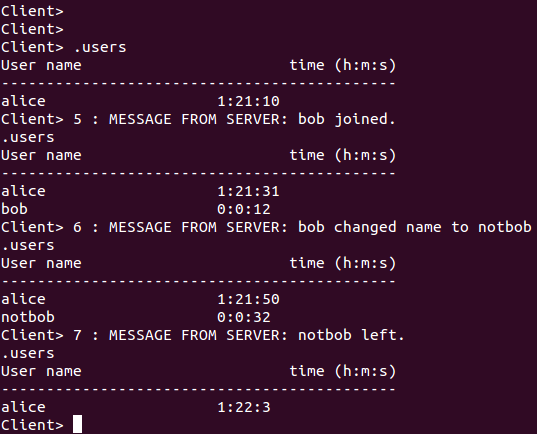
\includegraphics[scale=0.5]{conversation}
	\caption{Output from Alice's chatclient. Alice uses \textbf{.users} to see who's online. She also receives notifications when Bob connects, changes his name to notbob, and disconnects.}
	\label{testalicebob}
\end{figure}

\end{document}


